\documentclass[12pt]{article}
\usepackage{graphicx} % Required for inserting images
\usepackage[T2A]{fontenc}
\usepackage[utf8]{inputenc}
\usepackage[russian]{babel} 

\usepackage{geometry}
\usepackage{minted}
\usepackage{amsmath}
\geometry{right=1.5 cm}
\geometry{left=2cm}
\geometry{top=2cm}
\geometry{bottom=2cm}
%\DeclareMathSizes{12}{30}{16}{12}
\DeclareMathSizes{10}{10.5}{7}{7}

\begin{document}

\begin{titlepage}	

	\begin{center}		

		Санкт-Петербургский Государственный Политехнический университет\\
		Высшая школа прикладной математики и вычислительной физики\\
		Дисциплина "Математическая статистика"\\[6cm]

		\huge {Отчёт по лабораторной работе №1} \\[6cm]


	\end{center} 
	\begin{flushright} 
		\begin{minipage}{0.3\textwidth} 
			\begin{flushleft} 

				\textbf{Работу выполнил:}\\
				{Крупица С.В.}\\
				{Группа:  5030102/20101} \\

				\textbf{Преподаватель:}\\
				{Баженов А.Н.}\\

			\end{flushleft}
		\end{minipage}
	\end{flushright}

	\vfill 
\end{titlepage}

\newpage
\tableofcontents
\newpage
\section{Формулировка задания}
Для 4 распределений:
\begin{itemize}
    \item Нормальное распределение N(x,0,1)
    \item Распределение Коши C(x,0,1)
    \item Распределение Пуассона P(k,1,0)
    \item Равномерное распределение U(x,$-\sqrt{√3}$,$\sqrt{√3}$)
    
\end{itemize}


\begin{enumerate}
    \item  Сгенерировать выборки размером 10, 50 и 1000 элементов.
 Построить на одном рисунке гистограмму и график плотности рас
пределения.
    \item Сгенерировать выборки размером 10, 100 и 1000 элементов.
 Для каждой выборки вычислить следующие статистические характе ристики положения данных: $\hat{x}, med x, z_Q$. 
 Повторить такие вычисления 1000 раз для каждой выборки и найти среднее характеристик положения и их квадратов.
\end{enumerate}

\section{Полученные данные}
В данной таблице представленные все необходимые данные для каждого распределения и каждой выборки:\\
\begin{tabular}{|c|l|l|l|l|l|l|l|l|}
	\hline
	Распределение & Выборка & $\overline{x}$ & $med(x)$  & $z_q$ & $\overline{x^2}$ & $med(x^2)$ & $z_q^2$ & $D(x)$ \\
	\hline
	Коши & 10 & -0.8592 & 0.0228 & -0.0012 & 1729.3039 & 0.3715 & 0.8725 & 1728.5657 \\
	\hline
	   \ & 50 & 0.7522 & 0.0046 & 0.0051 & 2385.0325 & 0.0562 & 0.1127 & 2384.4667 \\
	\hline
	   \ & 1000 & 0.1350 & 0.0008 & -0.0010 & 948.2135 & 0.0023 & 0.0052 & 948.1953 \\
	\hline
		Нормальное & 10 & -0.0154 & -0.0265 & -0.0120 & 0.0943 & 0.1341 & 0.1051 & 0.0941 \\
	\hline
		\ & 50 & 0.0057 & 0.0073 & 0.0029 & 0.0190 & 0.0281 & 0.0230 & 0.0189 \\
	\hline
		\ & 1000 & -0.0014 & -0.0019 & -0.0005 & 0.0010 & 0.0016 & 0.0013 & 0.0010 \\
	\hline
		Пуассоновское & 10 & 10.0021 & 9.8635 & 9.9340 & 101.0023 & 98.7053 & 99.8338 & 0.9603 \\
	\hline
		\ & 50 & 9.9966 & 9.8255 & 9.8948 & 100.1278 & 96.8713 & 98.1694 & 0.1958 \\
	\hline
		\ & 1000 & 9.9986 & 9.9945 & 9.9949 & 99.9826 & 99.8953 & 99.9003 & 0.0100 \\
	\hline
		Равномерное & 10 & 0.0069 & 0.0096 & 0.0062 & 0.1004 & 0.2318 & 0.1423 & 0.1004 \\
	\hline
		\ & 50 & 0.0008 & 0.0047 & -0.0012 & 0.0205 & 0.0579 & 0.0301 & 0.0205 \\
	\hline
		\ & 1000 & -0.0018 & -0.0033 & -0.0016 & 0.0010 & 0.0030 & 0.0015 & 0.0010 \\
	\hline

\end{tabular}

\section{Графики}

\begin{center}
    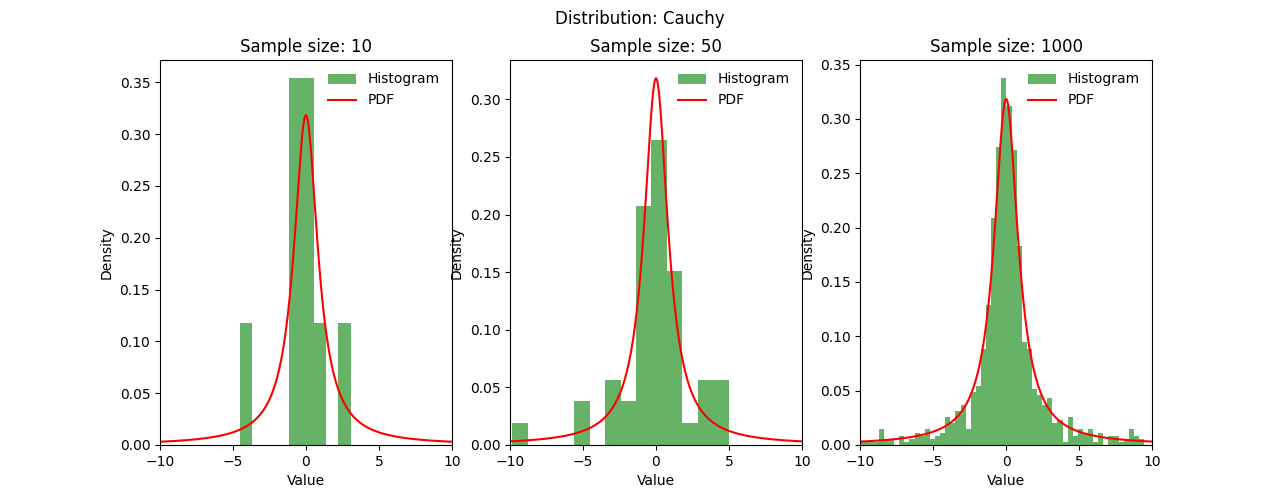
\includegraphics[scale=0.65]{lab_1_Cauchy.png} \\
    Рис. 1 График распределения Коши
\end{center}

\begin{center}
    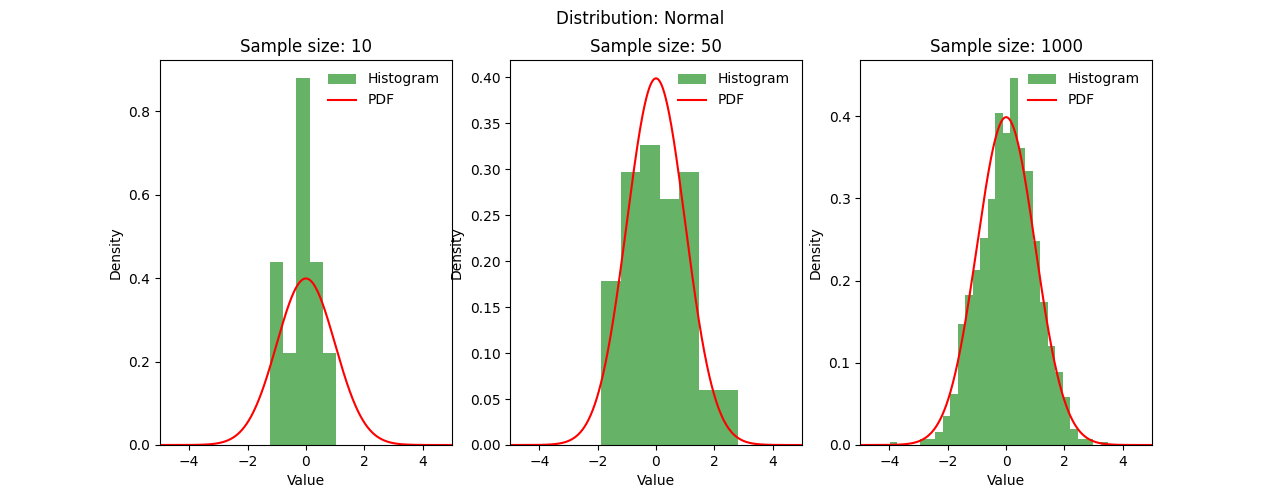
\includegraphics[scale=0.65]{lab_1_Normal.png} \\
    Рис. 2 График нормального распределения
\end{center}

\begin{center}
    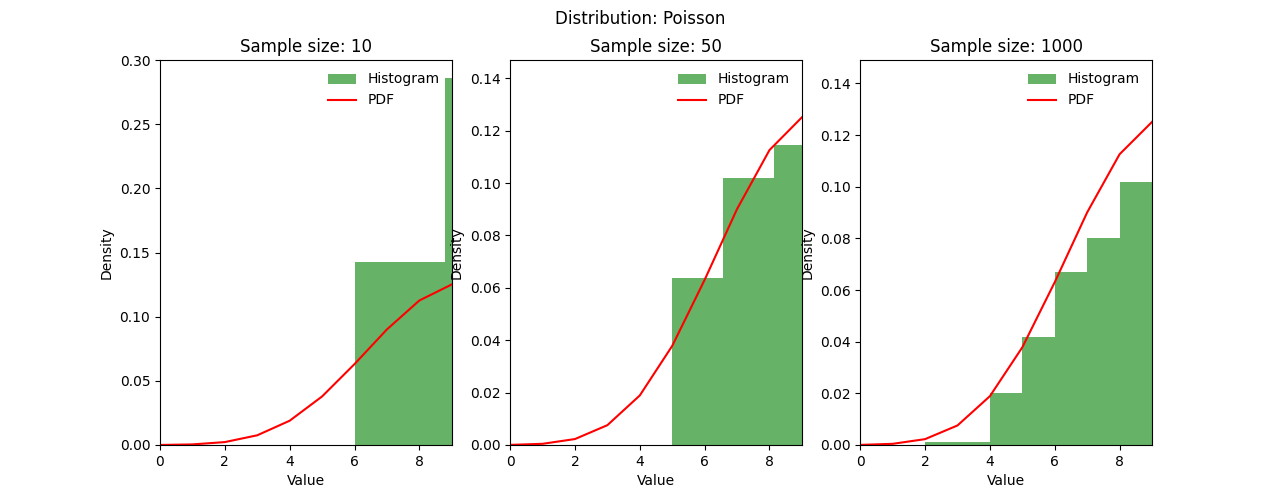
\includegraphics[scale=0.65]{lab_1_Poisson.png} \\
    Рис. 3 График распределения Пуассона
\end{center}

\begin{center}
    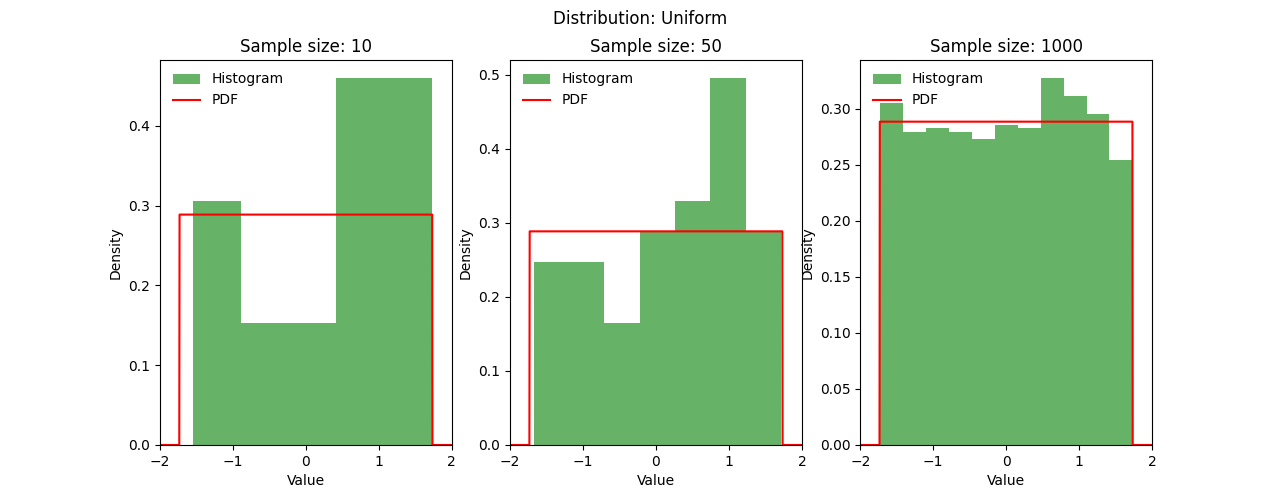
\includegraphics[scale=0.65]{lab_1_Uniform.png} \\
    Рис. 4 График равномерного распределения
\end{center}

\section{Вывод}
Не совсем понятно, что говорить в выводе. Исходя из данных таблицы и графиков, можно сделать вывод, что чем больше размер нашей выборки, тем меньше дисперсия, то есть отклонение практических результатов от теоретического значения. Это ровно то, что мы и ждем на практике исходя из закона больших чисел


\section*{Приложение: Ссылка на GitHub}


\url{https://github.com/ivgl/MatStatistic}

\end{document}
